\documentclass{article}
\usepackage[headheight=40pt, textheight=560pt]{geometry}
\usepackage{paralist}
\usepackage{scalerel,amssymb}
\usepackage{amsmath}
\usepackage{colortbl}
\usepackage{array}
\usepackage{multirow}
\usepackage{blindtext}
\usepackage{reledmac}
\usepackage{changepage}

\usepackage{pgfplots}
\usepackage{tikz}
\usetikzlibrary{positioning}
\usetikzlibrary{shapes.geometric, arrows}
\tikzstyle{arrow} = [thick,->,>=stealth]

\usepackage{graphicx}
\usepackage{stix}

\newcommand{\tableflip}{$($\rotatebox{45}{$\smile$}$^{\circ}\smwhtsquare^{\circ})\rotatebox{45}{$\smile$}\mkern-6mu\frown$\raisebox{0.5ex}{$\bot$}$\mkern-3.5mu-\mkern-3.5mu$\raisebox{0.5ex}{$\bot$}}

\usepackage{stackengine}
\def\apeqA{\SavedStyle\sim}
\def\apeq{\setstackgap{L}{\dimexpr.5pt+1.5\LMpt}\ensurestackMath{%
  \ThisStyle{\mathrel{\Centerstack{{\apeqA} {\apeqA} {\apeqA}}}}}}

\usepackage{fancyhdr}
\fancyhead[L]{
	\begin{tabular}{ll}
		\begin{tabular}{l}
			%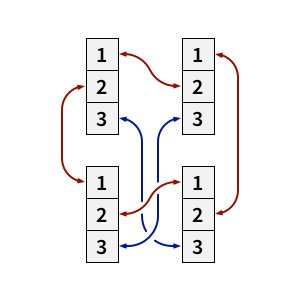
\includegraphics[scale=0.13]{distributed}
		\end{tabular}	
		&
		\begin{tabular}{l}
			\LARGE \textbf{Wirtschaftsinformatik} \\
			\Large \textsc{Fragen}
		\end{tabular}
	\end{tabular}
}
\fancyhead[R]{
	\begin{tabular}{r}
		16-124-836 \\
		Marcel \textsc{Zauder}
	\end{tabular}
}
\renewcommand{\headrulewidth}{0.4pt}
\fancyfoot[L]{\hspace{2cm}\thepage}
\fancyfoot[C]{}
\fancyfoot[R]{Informationstechnologie}
\renewcommand{\footrulewidth}{0.4pt}

\usepackage{hyperref}

\begin{document}
	\pagestyle{fancy}
	
	\section*{Teil 01: Informationstechnologie}
	\begin{adjustwidth}{2em}{2em}
		\section{Wirtschaftsinformatik und das digitalisierte Unternehmen}
		\begin{adjustwidth}{2em}{2em}
			\subsection{Sie haben einen Eindruck, was unter Digitaler Transformation zu verstehen ist}
			\begin{adjustwidth}{1em}{}
				\subsubsection*{Question: Welchen Aussagen bezüglich der digitalen Transformation stimmen Sie zu?}
				\begin{adjustwidth}{1em}{}
					\begin{enumerate}[(a)]
						\item Das Medium Papier wird von digitalen Dokumenten ersetzt und wird dadurch häufig verdrängt.
						\item Die Prozesse werden durch diese Umstellung häufig verändert und angepasst.
						\item Das digitalisierte Dokument kann mit weiteren Informationen versehen werden und besitzt ein deutlich größeres Anwendungsspektrum als das Medium Papier (zum Beispiel, wer hat Zugriff auf das Dokument oder auf Teie der Informationen).
						\item Ein Beispiel für digitale Transformation ist die Verbreitung von Vorlesungsinformationen, welche heute fast ausschließlich durch das Internet erfolgt und dadurch auch mehr Möglichkeiten bietet.
					\end{enumerate}
				\end{adjustwidth}
			\end{adjustwidth}
			\subsection{Sie verstehen die Problematik bei der Übertragung herkömmlicher Konzepte auf digitale Artefakte}
			\begin{adjustwidth}{1em}{}
				\subsubsection*{Question: Welche Probleme bringt die digitale Transformation mit sich?}
				\begin{adjustwidth}{1em}{}
					\begin{enumerate}[(a)]
						\item Die zu digitalisierenden Daten müssen eventuell aufwändig aufbereitet werden, um sie in digitaler Form nutzbar zu machen.
						\item Der Umgang mit diesen Daten und die neu entstandenen Prozesse müssen erläutert und gelehrt werden.
						\item Neue Technik (eventuell auch sehr teure) muss angeschafft werden, um die Daten verarbeiten zu können.
						\item Bei einer ganz neuen Implementation sind nicht alle zukünftigen Probleme direkt ersichtlich (Beispiel: Bandbreite für Server kann in Zukunft zu klein sein)
					\end{enumerate}
				\end{adjustwidth}
			\end{adjustwidth}
			\subsection{Sie können Wirtschaftsinformatik als Teilgebiet der Betriebswirtschaftslehre definieren}
			\begin{adjustwidth}{1em}{}
				\subsubsection*{Question: Was ist das Ziel der Wirtschaftsinformatik?}
				\begin{adjustwidth}{1em}{}
					\begin{enumerate}[(a)]
						\item Die Wirtschaftsinformatik kann dem Menschen Werkzeuge bieten und ihm bei verschiedenen Aufgaben unterstützen.
						\item Die Elemente der Wirtschaftsinformatik können mit dem Menschen arbeitsteilig kollaborieren.
						\item Durch die Wirtschaftsinformatik werden Betriebsprozesse digitalisiert und automatisiert (substituiert).
						\item Die Einführung von Wirtschaftsinformatik kann die betriebswirtschaftlichen Handlungen vereinfachen, den Aufwand verringern und das Ergebnis verbessern.
					\end{enumerate}
				\end{adjustwidth}
			\end{adjustwidth}
			\subsection{Sie wissen, dass Informationssysteme sowohl manuell als auch rechnerbasiert aufgebaut sein können}
			\begin{adjustwidth}{1em}{}
				\subsubsection*{Question: Was ist unter dem Begriff Informationssystem zu verstehen?}
				\begin{adjustwidth}{1em}{}
					\begin{enumerate}[(a)]
						\item Einem Informationssystem können durch einen Input Informationen bereitgestellt werden.
						\item Ein Informationssystem verarbeitet die bereitgestellten Informationen (Transformation von Daten). 
						\item Das Ergebnis der Verarbeitung wird als Output ausgegeben.
						\item Sowohl Mensch als auch Maschine können als solch ein Informationssystem aufgefasst werden.
					\end{enumerate}
				\end{adjustwidth}
			\end{adjustwidth}
			\subsection{Sie wissen, was ein sozio-technisches System ist}
			\begin{adjustwidth}{1em}{}
				\subsubsection*{Question: Was sind die Aspekte eines sozio-technischen Systems?}
				\begin{adjustwidth}{1em}{}
					\begin{enumerate}[(a)]
						\item Bei einem sozio-technischen System werden menschliche und maschinelle Komponenten, welche voneinander unabhängig sind, zusammengebracht, um eine Aufgabe zu erfüllen.
						\item Das soziale System und das technische System arbeiten bei der Abwicklung von Aufgaben zusammen und greifen ineinander über.
						\item Im Mittelpunkt steht die Unterstützung bei der Erfüllung von betrieblichen Aufgaben.
						\item Ein Beispiel für ein soziotechnisches System sind Informations- und Kommunikationssysteme.
					\end{enumerate}
				\end{adjustwidth}
			\end{adjustwidth}
			\subsection{Sie kennen verschiedene Perspektiven auf den IKT-Einsatz}
			\begin{adjustwidth}{1em}{}
				\subsubsection*{Question: Welche Aufgaben besitzt die IKT in Bezug auf einen Betrieb?}
				\begin{adjustwidth}{1em}{}
					\begin{enumerate}[(a)]
						\item Die IKT unterstützt die Übermittlung von Informationen.
						\item Die IKT kann Informationen persistent speichern, welche erst in Zukunft gebraucht werden.
						\item Die IKT beinhaltet einen Algorithmus, um Informationen umzuformen, damit diese einfacher gehandhabt werden können (zum Beispiel, um sie einfach auslesbar zu machen).
						\item Die IKT besitzt weitere Komponenten, um bei der Erfüllung von Prozessen unterstützend mitzuwirken.
					\end{enumerate}
				\end{adjustwidth}
			\end{adjustwidth}
		\end{adjustwidth}
		
		\section{Grundlagen Rechner, Befehle und Daten}
		\begin{adjustwidth}{2em}{2em}
			\subsection{Sie wissen, welche Hauptkomponenten bei der Verarbeitung in einem Rechner eine Rolle spielen}
			\begin{adjustwidth}{1em}{}
				\subsubsection*{Question: Welche Hauptkomponenten sind bei der Verarbeitung in einem Rechner wichtig?}
				\begin{adjustwidth}{1em}{}
					\begin{enumerate}[(a)]
						\item Steuerwerk im Prozessor - kontrolliert den Ablauf und die Ausführung der Befehle
						\item Rechenwerk im Prozessor - verarbeitet die Elementarbefehle, welche vom Steuerwerk vorgegeben werden mit den Informationen aus dem Hauptspeicher
						\item Hauptspeicher - beinhaltet verschiedene Speicherzellen, in welchen die Informationen und Elementarbefehle abgespeichert sind.
						\item Input- und Output-Geräte werden für die Interaktion mit dem Nutzer genutzt.
					\end{enumerate}
				\end{adjustwidth}
			\end{adjustwidth}
			\subsection{Sie kennen Prozessoren und Speicherchips als relevante integrierte Schaltkreise}
			\begin{adjustwidth}{1em}{}
				\subsubsection*{Question: Welchen Aussagen über Prozessoren und Speicherchips stimmen Sie zu?}
				\begin{adjustwidth}{1em}{}
					\begin{enumerate}[(a)]
						\item Speicherchips enthalten einzeln addressierbare Speicherzellen von 32 oder 64 Bit.
						\item Der Prozessor ist die wichtigste Komponente eines Rechners, da hier alle Programme und Befehle ausgeführt werden.
						\item Ein Prozessor besitzt ein Steuerwerk, welches die Ausführung der Anweisungen kontrolliert.
						\item Ein Prozessor besitzt ein Rechenwerk, welche die Elemtaroperationen, wie Addition, AND oder OR, durchführt.
					\end{enumerate}
				\end{adjustwidth}
			\end{adjustwidth}
			\subsection{Sie können das Moore'sche Gesetz und dessen Bedeutung beschreiben}
			\begin{adjustwidth}{1em}{}
				\subsubsection*{Question: Was beschreibt das Moore'sche Gesetz und welche Folgen hat dies auf die technische Welt?}
				\begin{adjustwidth}{1em}{}
					\begin{enumerate}[(a)]
						\item Die Anzahl der Transistoren auf einem integrierten Schaltkreis verdoppelt sich in regelmäßigen Abständen.
						\item Dadurch können leistungsfähigere Rechner bei ungefähr gleichbleibenden Kosten hergestellt werden.
						\item Die Rechengeschwindigkeit von Computern verdoppelt sich somit auch in regelmäßigen Abständen
						\item Die Speicherkapazität von Speicherchips verdoppelt sich somit auch in regelmäßigen Abständen
					\end{enumerate}
				\end{adjustwidth}
			\end{adjustwidth}
			\subsection{Sie wissen, dass zwischen der Menschenwelt und der binären Maschinenwelt Übersetzungen und Umcodierungen stattfinden müssen}
			\begin{adjustwidth}{1em}{}
				\subsubsection*{Question: Welche Probleme ergeben sich wenn eine Person mit einem Computer kommunizieren will?}
				\begin{adjustwidth}{1em}{}
					\begin{enumerate}[(a)]
						\item Eine Person benutzt Wörter, um sich zu verständigen. Ein Computer kennt die Bedeutung dieser Wörter nicht.
						\item Ein Rechner verwendet die Binärdarstellung (Nullen und Einsen), um Informationen und Befehlssätze abzubilden. Dies wiederum kann eine Person nicht direkt verstehen.
						\item Die Daten- und Befehlseingabe einer Person muss übersetzt werden, damit der Rechner weiß was durchgeführt werden soll.
						\item Der Output eines Rechners muss so aufgearbeitet werden, dass die Person die Informationen auslesen und verstehen kann.
					\end{enumerate}
				\end{adjustwidth}
			\end{adjustwidth}
			\subsection{Sie kennen den Unterschied zwischen Maschinencode, Assembler und höheren Programmiersprachen}
			\begin{adjustwidth}{1em}{}
				\subsubsection*{Question: Welchen Aussagen über die verschiedenen Programmiersprachen stimmen Sie zu?}
				\begin{adjustwidth}{1em}{}
					\begin{enumerate}[(a)]
						\item Die Maschinensprache beinhaltet direkte Anweisungen an den Prozessor in Maschinencode (Nullen und Einsen).
						\item Die Assemblersprache besitzt Befehlskürzel (Mnemonics), welche die direkten Anweisungen an den Prozessor abbilden und verständlicher für den Menschen sind als der Maschinencode.
						\item Eine höhere Programmiersprache orientiert sich an der menschlichen Logik und ist losgelöst vom Prozessor.
						\item Die höhere Programmiersprache beinhaltet mächtige Befehle, welche von Personen sehr einfach verstanden werden kann.
					\end{enumerate}
				\end{adjustwidth}
			\end{adjustwidth}
			\subsection{Sie wissen was ein Datentyp ist und können Codierungen für verschiedene Datentypen erklären}
			\begin{adjustwidth}{1em}{}
				\subsubsection*{Question: Wieso müssen zur Datenverarbeitung verschiedene Datentypen vorhanden sein?}
				\begin{adjustwidth}{1em}{}
					\begin{enumerate}[(a)]
						\item Jede Art von Information/Daten werden binär im Speicher abgelegt. Ohne Definition des Datentyps kann nicht entschieden werden, ob es sich bei der Information um eine Ganze Zahl, Text oder anderem handelt.
						\item Jeder Datentyp wird daher unterschiedlich codiert
						\item Der Datentyp bestimmt, welche Daten und welche Operationen mit den Daten zulässig sind, wie auch wie sie im Computer und dem Benutzer dargestellt werden.
						\item Daten müssen einem Datentyp zugewiesen werden, damit der Rechner weiß was er mit diesen Daten machen kann.
					\end{enumerate}
				\end{adjustwidth}
			\end{adjustwidth}
			\subsection{Sie können Probleme nennen, die bei der Verwendung verschiedener Datentypen auftreten können}
			\begin{adjustwidth}{1em}{}
				\subsubsection*{Question: Welche Probleme können bei der Verwendung verschiedener Datentypen auftreten?}
				\begin{adjustwidth}{1em}{}
					\begin{enumerate}[(a)]
						\item Der Datentyp Integer besitzt eine obere Grenze, wodurch bei Überschreitung dieser Grenze ein Überlaufproblem entsteht, wodurch das Vorzeichen der Zahl wechselt (Beispiel: bei einem 32-Bit-Integer ist der maximal zulässige Wert 2.147.283.647).
						\item Bei einer Festkommzahl ist die Position des Kommas und die Anzahl von Ziffern fest vorgegeben. Damit ist die Darstellung einer Zahl nur im gesamten Wertebereich exakt.
						\item Bei Gleitkommazahlen erfolgt eine angenäherte Darstellung einer reellen Zahl, wodurch die Werte nicht immer ganz exakt sind (aber der Wertebereich ist nicht begrenzt)
						\item Bei der Darstellung von Zeichen wird der ISO 7-bit Code benutzt. Dieser besitzt aber keine Umlaute und nicht alle Spezialzeichen (da dieser in den USA "erfunden" wurde). Daher muss der Zeichensatz mit weiteren Einträgen erweitert werden, damit Zeichen wie 'Ü' usw. abgebildet werden können. Andernfalls werden sie vom System nicht richtig interpretiert.
					\end{enumerate}
				\end{adjustwidth}
			\end{adjustwidth}
		\end{adjustwidth}
		
		\newpage		
		
		\section{Typen von Software}
		\begin{adjustwidth}{2em}{2em}
			\subsection{Sie kennen den Unterschied von Systemsoftware und Anwendungssoftware}
			\begin{adjustwidth}{1em}{}
				\subsubsection*{Question: Was ist der Unterschied zwischen Systemsoftware und Anwendungssoftware?}
				\begin{adjustwidth}{1em}{}
					\begin{enumerate}[(a)]
						\item Die Systemsoftware bietet eine Plattform für andere Software, indem es eine Verbindung zur Hardware herstellt und die Verwendung von Ressourcen steuert.
						\item Hauptsächlich gehören vor allem Betriebssysteme oder auch systemnahe Software zur Systemsoftware.
						\item Eine Anwendungssoftware unterstützen den Benutzer beim Durchführen von Geschäftsprozessen und betrieblichen Anwendungen.
						\item Anwendungssoftware bietet eine Anwendung von Informations- und Kommunikationstechnologien auf (betriebliche=) Aufgabenstellungen.
					\end{enumerate}
				\end{adjustwidth}
			\end{adjustwidth}
			\subsection{Sie wissen, welche Aufgaben ein Betriebssystem übernimmt}
			\begin{adjustwidth}{1em}{}
				\subsubsection*{Question: Für welche Aufgaben ist ein Betriebssystem zuständig?}
				\begin{adjustwidth}{1em}{}
					\begin{enumerate}[(a)]
						\item Das Betriebssystem erzeugt ein leichter verständliche Schnittstelle zur eigentlichen Maschine, damit der Benutzer die Betriebsmittel besser handhaben kann.
						\item Das Betriebssystem ordnet Input/Output-Geräte den jeweiligen Allokationen zu und verwaltet alle weiteren Hardwareressourcen.
						\item Ein Betriebssystem überwacht außerdem welches Programm welche Betriebsmittel nutzt.
						\item Das Betriebssystem verdeckt und vereinfacht die Komplexität der Maschine durch Erzeugung von abstrakten Objekten.
					\end{enumerate}
				\end{adjustwidth}
			\end{adjustwidth}
			\subsection{Sie können einen Überblick über drei verschiedene Typen betrieblicher Anwendungssystem geben}
			\begin{adjustwidth}{1em}{}
				\subsubsection*{Question: Wie werden Anwendungssystem in einem Betrieb genutzt?}
				\begin{adjustwidth}{1em}{}
					\begin{enumerate}[(a)]
						\item Büroinformationssysteme unterstützen die typische Büroarbeit und beinhaltet verschieden Werkzeuge zur Individuellen- und Gruppenunterstützung.
						\item Büroinformationssystem beinhalten häufig kollaborative Funktionen, wie zum Beispiel Daten- und Informationsaustausch.
						\item Transaktionssysteme, wie ERP, sind häufig eine Ansammlung von Applikationen, welche genutzt werden, um den ganzen Betrieb zu verwalten. Ein verteiltes Datenbanksystem beinhaltet alle Informationen, welche in dem Betrieb anfallen.
						\item Manegementunterstützungssysteme versorgen Führungskräfte mit Informationen und helfen bei der Entscheidungsfindung.
					\end{enumerate}
				\end{adjustwidth}
			\end{adjustwidth}
			\subsection{Sie können Individualsoftware und Standardsoftware unterscheiden}
			\begin{adjustwidth}{1em}{}
				\subsubsection*{Question: Was ist der Unterschied zwischen Individual- und Standardsoftware?}
				\begin{adjustwidth}{1em}{}
					\begin{enumerate}[(a)]
						\item Individualsoftware wird auf die Bedürfnisse eines Kunden angepasst und entwickelt.
						\item Dadurch entspricht die Individualsoftware genau den Anforderungen des Anwenders, ist aber dadurch auch sehr teuer .
						\item Standardsoftware besitzt viele verschiedene Funktionen, um einen Großteil bestimmter funktionaler Anforderungen für einen breiten Kreis von Anwendern abzudecken
						\item Dadurch verteilen sich die Kosten für (Weiter-)Entwicklung auf viele verschiedene Anwender und ist dadurch günstiger. Es kann dennoch vorkommen, dass nicht alle Anforderungen des Nutzers genau abgedeckt werden.
					\end{enumerate}
				\end{adjustwidth}
			\end{adjustwidth}
			\subsection{Sie kennen die Argumente die für und gegen Standardsoftware sprechen.}
			\begin{adjustwidth}{1em}{}
				\subsubsection*{Question: Was sind Vor- und Nachteil von Standardsoftware?}
				\begin{adjustwidth}{1em}{}
					\begin{enumerate}[(a)]
						\item Die (Weiter-)Entwicklungkosten werden auf viele verschiedene Anwender verteilt, wodurch sie für den einzelnen günstiger ist.
						\item Durch die vielen verschiedenen Nutzer können Probleme schneller entdeckt werden und alle Nutzer profitieren von den Erfahrungen anderer Nutzer
						\item Sie kann schneller eingeführt werden, da die Software bereits besteht und eventuell schon von vielen anderen Betrieben eingeführt wurde.
						\item Standardsoftware deckt nicht unbedingt alle Anforderungen des einzelnen Nutzers ab.
					\end{enumerate}
				\end{adjustwidth}
			\end{adjustwidth}
			\subsection{Sie wissen, was Open Source Software ist und kennen die Bedeutung von Lizenzen bei der Nutzung von Software}
			\begin{adjustwidth}{1em}{}
				\subsubsection*{Question: Was sind Lizenzen und welche spezielle Stellung hat die Open Source Software bezüglich dieser?}
				\begin{adjustwidth}{1em}{}
					\begin{enumerate}[(a)]
						\item Lizenzen erlauben die Nutzung der Software. In dieser sind eventuell auch Einschränkung in Bezug auf die Nutzung und Weitergabe dieser definiert.
						\item Die Veränderung von lizenzierten Produkten ist normalerweise ausgeschlossen, da der Quell-Code nicht offengelegt wird.
						\item Bei Open Source Software wird der Quellcode offen gelegt und darf beliebig verändert, eingesetzt und verbreitet werden.
						\item Die Nutzung von Open Source Software ist auch an bestimmte Lizenzen gebunden, welche aber normalerweise weniger strikt sind als die von Proprietärer Software.
					\end{enumerate}
				\end{adjustwidth}
			\end{adjustwidth}
			\subsection{Sie kennen das Konzept Total Cost of Ownership und welche Rolle es bei der Beurteilung von Open Source Software spielt}
			\begin{adjustwidth}{1em}{}
				\subsubsection*{Question: Was ist das Konzept Total Cost of Ownership und wie wirkt sie sich auf die Beurteilung von Open Source Software aus?}
				\begin{adjustwidth}{1em}{}
					\begin{enumerate}[(a)]
						\item Die Total Cost of Ownership bietet einen ganzheitlichen Überblick über die Informatikkosten.
						\item Durch die TCO wird versucht unterschiedliche IT-Produkte vergleichbar zu machen. Hier steht vor allem im Vordergrund Proprietäre Software versus Open Source.
						\item Der Vorteil von Open Source Software im Hinblick auf die TCO ist dass die Lizenzgebühren für diese deutlich günstiger sind als bei der Proprietären Software.
						\item Der Nachteil von OSS ist dagegen die unbekannten Kosten welche durch (un)geplante Downtime oder durch Einführung/Umschulung anfallen.
					\end{enumerate}
				\end{adjustwidth}
			\end{adjustwidth}
		\end{adjustwidth}
		
		\newpage		
		
		\section{Vernetzte Rechner-Infrastruktur}
		\begin{adjustwidth}{2em}{2em}
			\subsection{Sie kennen den Unterschied zwischen einer zentralen und einer dezentralen Datenverarbeitung}
			\begin{adjustwidth}{1em}{}
				\subsubsection*{Question: Wie unterscheiden sich eine zentrale und eine dezentrale Datenverarbeitung voneinander?}
				\begin{adjustwidth}{1em}{}
					\begin{enumerate}[(a)]
						\item Bei der zentralisierten Datenverarbeitung werden Großrechner benutzt, welche in speziell ausgerüsteten Rechenzentren zusammengefasst sind.
						\item Mehrere Benutzer können auf solch einem Großrechner arbeiten und unterschiedliche Programme nutzen. Dabei benutzen sie Terminals, welche keine eigenständige Verarbeitungskapazität besitzt.
						\item Durch die Einführung von Personal Computern kann der Benutzer auf seinem eigenen Gerät mit einer eigenständigen Verarbeitungskapazität arbeiten.
						\item Diese wurden vor allem zur Unterstützung von Büro-Tätigkeiten eingesetzt.
					\end{enumerate}
				\end{adjustwidth}
			\end{adjustwidth}
			\subsection{Sie wissen um die Rolle von Rechnernetzen bei der Realisierung von dezentralen Datenverarbeitung}
			\begin{adjustwidth}{1em}{}
				\subsubsection*{Question: Welche Rolle spielen Rechnersysteme bei der Realisierung von dezentralen DV?}
				\begin{adjustwidth}{1em}{}
					\begin{enumerate}[(a)]
						\item Alleinstehende Computer wurden in einem Rechnernetz zusammengeschlossen, um die Ressourcen gemeinsam nutzbar zu machen.
						\item Durch diese Rechnernetze können Daten und Informationen schnell ausgetauscht werden
						\item Durch die vernetzte DV können zum Beispiel Drucker oder auch Speichermedien jedem zugänglich gemacht werden.
						\item Einzelne Computer in solchen Rechnernetzen können auch arbeitsteilig zusammeenarbeiten und Aufgaben schneller zu erfüllen.
					\end{enumerate}
				\end{adjustwidth}
			\end{adjustwidth}
			\subsection{Sie bekommen einen Einblick in das Client-Server-Prinzip}
			\begin{adjustwidth}{1em}{}
				\subsubsection*{Question: Was versteht man unter dem Client-Server-Prinzip?}
				\begin{adjustwidth}{1em}{}
					\begin{enumerate}[(a)]
						\item Beim Client-Server-Prinzip werden die ausführbaren Programme in Client und Server unterschieden
						\item Jeder Client kann einen Serverdienst anfragen.
						\item Der Server stellt einen Dienst passend den Anforderungen des Clients bereit.
						\item Ein Server kann dabei mehrere Clients gleichzeitig bearbeiten.
					\end{enumerate}
				\end{adjustwidth}
			\end{adjustwidth}
			\subsection{Sie können einen Server als Software-Komponente von einem Server als Rechner abgrenzen}
			\begin{adjustwidth}{1em}{}
				\subsubsection*{Question: Was ist der Unterschied zwischen einem Server als Software-Komponente und einem Server als Rechner?}
				\begin{adjustwidth}{1em}{}
					\begin{enumerate}[(a)]
						\item Der Server als Software-Komponente ist ein Programm, welches anderen Programmen Dienste zur Verfügung stellt
						\item Der Server als Software-Komponente bearbeitet Anfragen von Client-Programmen
						\item Der Server als Rechner kann viele verschiedene Server-Funktionen übernehmen
						\item ...
					\end{enumerate}
				\end{adjustwidth}
			\end{adjustwidth}
			\subsection{Sie haben einen Überblick über moderne IT-Infrastrukturen}
			\begin{adjustwidth}{1em}{}
				\subsubsection*{Question: Was sind heutzutage die wichtigsten Aspekte der IT-Infrastruktur?}
				\begin{adjustwidth}{1em}{}
					\begin{enumerate}[(a)]
						\item Dadurch dass heutzutage viele Mitarbeiter auch private mobile Geräte wie Laptops oder ähnlichem besitzen, können diese auch bei der Arbeit genutzt werden.
						\item Um auch andere mobile Geräte nutzbar zu machen, werden Server benutzt, welche verschiedene Applikation und Komponenten als Dienstleistung anbieten.
						\item Um Daten betriebsintern abspeichern zu können, werden Storage-System genutzt welche direkt an das betriebsinterne Netzwerk angehängt werden.
						\item Auch der sichere Betrieb der einzelnen Komponenten spielt eine wichtige Rolle in der IT-Infrastruktur und erfordert bestimmte Voraussetzungen wie Klimatisierung, Schutzanlagen und Sicherheitssysteme.
					\end{enumerate}
				\end{adjustwidth}
			\end{adjustwidth}
			\subsection{Sie wissen, welche Ausprägungen des IT-Sourcing relevant sind}
			\begin{adjustwidth}{1em}{}
				\subsubsection*{Question: Welche Ausprägungen des IT-Sourcing sind heutzutage relevant?}
				\begin{adjustwidth}{1em}{}
					\begin{enumerate}[(a)]
						\item Beim Server-Housing steht der zu betreibende Server in einem professionellem Rechenzentrum.
						\item Einzelne Applikation oder sogar die ganze Informatikabteilung können extern betrieben werden (Outsourcing)
						\item Die IT-Ressourcen werden als Dienstleistung über das Internet bereitgestellt (Cloud-Computing)
						\item Das Cloud-Computing kann unterschiedliche Schichten des Systemstapels betreffen (von Software bis Infrastruktur).
					\end{enumerate}
				\end{adjustwidth}
			\end{adjustwidth}
			\subsection{Sie kennen das Konzept des Cloud Computing}
			\begin{adjustwidth}{1em}{}
				\subsubsection*{Question: Welche verschiedenen Arten des Cloud Computings gibt es?}
				\begin{adjustwidth}{1em}{}
					\begin{enumerate}[(a)]
						\item Bei IaaS wird die Infrastruktur wie physische Server über das Internet als Dienstlesitung angeboten
						\item Bei PaaS werden zusätzlich unter anderem auch Betriebssysteme, Middleware bis hin zu Datenbanke angeboten.
						\item Bei SaaS werden alle Schichten des Systemstapels (bis hin zur Fachanwendung) als Dienstleistung angeboten.
						\item Wenn alle Komponenten des Systemstapels beim Nutzer selbst liegen spricht man von On-Premise.
					\end{enumerate}
				\end{adjustwidth}
			\end{adjustwidth}
		\end{adjustwidth}		
		
	\end{adjustwidth}
	
	\newpage
	\fancyfoot[R]{
		Daten und Prozesse
	}
	\setcounter{section}{0}
	\section*{Teil 02: Daten und Prozesse}
	\begin{adjustwidth}{2em}{2em}
		\section{Strukturierte und unstrukturierte Dateien}
		\begin{adjustwidth}{2em}{2em}
			\subsection{Sie haben einen Eindruck von der Analogie herkömmlicher Dokumentablagen und Dateiverwaltungssystemen}
			\begin{adjustwidth}{1em}{}
				\subsubsection*{Question: Wo liegen die Analogien zwischen der herkömmlichen Dokumentablage und dem Dateiverwaltungssystem?}
				\begin{adjustwidth}{1em}{}
					\begin{enumerate}[(a)]
						\item Beide können als eine Ablage für Aufzeichnungen gesehen werden, wobei es sich heute um ein digitales Dokument anstelle eines in Papierform handelt.
						\item Beide beinhalten eine Hierarchie der Dokumente und Dateien und können aufgrund dieser einfach zugeordnet werden.
						\item ...
						\item ...
					\end{enumerate}
				\end{adjustwidth}
			\end{adjustwidth}
			\subsection{Sie wissen, dass Dateien und Dateiverzeichnisse Abstraktionen von Betriebssysteme über Hardware-Komponenten sind}
			\begin{adjustwidth}{1em}{}
				\subsubsection*{Question: ...?}
				\begin{adjustwidth}{1em}{}
					\begin{enumerate}[(a)]
						\item ...
						\item ...
						\item ...
						\item ...
					\end{enumerate}
				\end{adjustwidth}
			\end{adjustwidth}
			\subsection{Sie kennen den Unterschied zwischen strukturierten und unstrukturierten Daten}
			\begin{adjustwidth}{1em}{}
				\subsubsection*{Question: Was sind die Unterschiede zwischen strukturierten und unstrukturierten Daten?}
				\begin{adjustwidth}{1em}{}
					\begin{enumerate}[(a)]
						\item Unstrukturierte Daten sind nicht in ihre Einzelteile aufgespalten werden und besitzen keine formale Struktur.
						\item Das automatische Verarbeiten von unstrukturierten Daten ist stark eingeschränkt.
						\item Strukturierte Daten erlauben den Zugriff auf bestimmte Teile und die Unterteilbarkeit in verschiedene kleinere Datenelemente.
						\item Strukturierte Daten können automatisch verarbeitet werden.
					\end{enumerate}
				\end{adjustwidth}
			\end{adjustwidth}
			\subsection{Sie wissen, wie der Zusammenhang zwischen Programmen und Dateien ist}
			\begin{adjustwidth}{1em}{}
				\subsubsection*{Question: Welchen Aussagen über den Zusammenhang zwischen Programmen und Dateien stimmen Sie zu?}
				\begin{adjustwidth}{1em}{}
					\begin{enumerate}[(a)]
						\item Dateien werden mit Hilfe von Anwendungsprogrammen verarbeitet und herkömmlicherweise auch verwaltet.
						\item Die Daten, welche verwendet werden, entsprechen den Anforderungen des Programms. 
						\item Daten besitzen allgemein bestimmte Dateiformate oder spezifische Datenstrukturen, welche vom Anwendungsprogramm verwaltet werden können.
						\item Ein Anwendungsprogramm kann in der Lage sein verschiedene Dateiformate zu verwenden.
					\end{enumerate}
				\end{adjustwidth}
			\end{adjustwidth}
			\subsection{Sie können Beispiele für die Nutzung von Dateiformaten durch verschiedene Programme nennen}
			\begin{adjustwidth}{1em}{}
				\subsubsection*{Question: Welche Unterschiede zwischen verschiedenen Dateiformate gibt es?}
				\begin{adjustwidth}{1em}{}
					\begin{enumerate}[(a)]
						\item Normale txt-Dateien sind eine reine Text-Datei welche nur den text an sich beinhaltet und keine weitere Formatinformationen.
						\item Eine XML-Datei beinhaltet Informationen zum Format der Textdatei, wie auch verschiedene Layout-Informationen
						\item Eine CSV beinhaltet Daten, welche durch ein bestimmtes Zeichen (wie ein Komma) separiert werden.
						\item XLSX oder XLS Datein können auch Formeln oder Formatierungen verwenden und verarbeiten.
					\end{enumerate}
				\end{adjustwidth}
			\end{adjustwidth}
			\subsection{Sie kennen das Konzept von Open Data}
			\begin{adjustwidth}{1em}{}
				\subsubsection*{Question: Was verbirgt sich hinter dem Begriff von Open Data?}
				\begin{adjustwidth}{1em}{}
					\begin{enumerate}[(a)]
						\item Open Data beschreibt ein Konzept, das erreichen soll, dass alle Daten im Internet offen gelegt werden und jeder Zugriff auf diese hat.
						\item Ähnlich wie Open Source sollen die Daten einfach und frei zugänglich sein. 
						\item Um verschiedene "Entwicklungsstufen" von Open Data zu differenzieren, wird das Five-Star-Modell genutzt.
						\item Open Data soll zu mehr Transparenz und Zusammenarbeit zwischen Personen/Abteilungen/Betrieben führen.
					\end{enumerate}
				\end{adjustwidth}
			\end{adjustwidth}
			\subsection{Sie können das Five-Star-Modell für die Eignung unterschiedlicher Dateiformate für Open Data beschreiben}
			\begin{adjustwidth}{1em}{}
				\subsubsection*{Question: Was sind Kriterien des Five-Star-Modell für Open Data?}
				\begin{adjustwidth}{1em}{}
					\begin{enumerate}[(a)]
						\item Die erste Stufe besagt, dass alle Daten in egal welcher Form im Web zugänglich sein sollen.
						\item Die zweite Stufe erweitert dies, sodass sich die Daten in einem strukturierten Format (wie eine Excel-Datei) befinden sollen.
						\item Die dritte Stufe besagt, dass es sich um nicht proprietäre Formate handeln soll (z.B. CSV anstelle von Excel).
						\item Die vierte Stufe verlangt, dass es möglich ist die Daten zu verlinken. Dies kann durch die Verwendung von URIs erreicht werden. 
					\end{enumerate}
				\end{adjustwidth}
			\end{adjustwidth}
		\end{adjustwidth}
			
		\newpage
			
		\section{Grundlagen relationaler Datenbanken}
		\begin{adjustwidth}{2em}{2em}
			\subsection{Sie kennen die Problematik dokumentorientierter Dateispeicherung}
			\begin{adjustwidth}{1em}{}
				\subsubsection*{Question: Welche Probleme bringt die dokumentorientierte Dateispeicherung mit sich?}
				\begin{adjustwidth}{1em}{}
					\begin{enumerate}[(a)]
						\item Verschiedene Dateien können dieselbe Information beinhalten, welche in unterschiedlichen Kontexten als Daten abgebildet sind.
						\item Verschiedene Dateien können redundante Informationen beinhalten.
						\item Redundante Informationen stellen ein Problem dar, wenn sich Daten verändern.
						\item Als Beispiel kann dieselbe Person mit unterschiedlichen Matrikelnummern in solch einer dokumentorientierten Dateispeicherung vorkommen.
					\end{enumerate}
				\end{adjustwidth}
			\end{adjustwidth}
			\subsection{Sie kennen das Konzept der logischen und physischen Datenunabhängigkeit}
			\begin{adjustwidth}{1em}{}
				\subsubsection*{Question: Was versteht man unter der logischen und physischen Datenunabhängigkeit?}
				\begin{adjustwidth}{1em}{}
					\begin{enumerate}[(a)]
						\item Die logische Datenunabhängigkeit besagt, dass die Verwaltung von Daten unabhängig vom jeweiligen Anwendungsprogramm, welches diese Daten benutzt, erfolgen soll
						\item Nur eine Änderung der Datenstruktur der Daten, welche direkt vom Anwendungsprogramm genutzt werden, erfordert auch eine Anpassung im Anwendungsprogramm selbst.
						\item Es spielt keine Rolle für die Verwaltung von Dateien, wie diese auf einem Speichermedium abgelegt sind.
						\item Eine Änderung auf dem Speichermedium erfordert keine Anpassung des (logischen) Datenschemas.
					\end{enumerate}
				\end{adjustwidth}
			\end{adjustwidth}
			\subsection{Sie wissen, das Datenbanksysteme häufig eine Client-Server-Architektur haben}
			\begin{adjustwidth}{1em}{}
				\subsubsection*{Question: Inwiefern beschreibt ein Datenbanksystem eine Client-Server-Architektur und welche Vorteile bringt dies mit sich?}
				\begin{adjustwidth}{1em}{}
					\begin{enumerate}[(a)]
						\item Datenbanksysteme sind heutzutage Teil der verteilten Datenverarbeitung.
						\item Die Datenbank mit dem dazugehörigen Datenbankmanagementsystem bilden die Serverkomponenten.
						\item Ein Programm kann als Client auf dieses Datenbankmanagementsystem zugreifen.
						\item Durch die Hinzunahme des Internets ist die Datenbank von überall erreichbar und führt daher auch zu einer flexibleren Nutzung von Daten.
					\end{enumerate}
				\end{adjustwidth}
			\end{adjustwidth}
			\subsection{Sie lernen die Eigenschaften des weit verbreiteten Relationalen Datenmodells kennen}
			\begin{adjustwidth}{1em}{}
				\subsubsection*{Question: Welche Vor- und Nachteile besitzt das Relationale Datenmodell?}
				\begin{adjustwidth}{1em}{}
					\begin{enumerate}[(a)]
						\item Das Relationale Datenmodell ist einfach, verständlich und flexibel.
						\item Es basiert auf der Mengentheorie und die zugrunde liegenden methodischen Grundlagen können so einfach gelehrt werden.
						\item Bei Einhaltung aller Normalformen werden Daten stark zerlegt und viel Tabellen erzeugt.
						\item Eine starke Zerlegung führt zu komplexen, unüberschaubaren Strukturen und ist vergleichsweise ressourcenintensiv.
					\end{enumerate}
				\end{adjustwidth}
			\end{adjustwidth}
			\subsection{Sie wissen, was mit elementaren Attributwerten gemeint ist und warum diese für Relationen wichtig sind}
			\begin{adjustwidth}{1em}{}
				\subsubsection*{Question: Was versteht man unter elementaren Attributwerten und wieso sind diese für Relationen wichtig?}
				\begin{adjustwidth}{1em}{}
					\begin{enumerate}[(a)]
						\item Dass ein Attributwert elementar sein muss, beschreibt dass nur ein Wert pro Zelle (Schnittpunkt von einer Zeile und einer Spalte) zulässig  ist.
						\item ...
						\item ...
						\item ...
					\end{enumerate}
				\end{adjustwidth}
			\end{adjustwidth}
			\subsection{Sie kennen den Unterschied zwischen Tabellen im Relationalen Datenmodell und in Tabellenkalkulationsprogrammen}
			\begin{adjustwidth}{1em}{}
				\subsubsection*{Question: Was ist der Unterschied zwischen Tabellen im Relationalem Datenmodell und in einem Tabellenkalkulationsprogramm?}
				\begin{adjustwidth}{1em}{}
					\begin{enumerate}[(a)]
						\item In einem Tabellenkalkulationsprogramm kann jede Zeile und jede Spalte über Indizes addressiert werden.
						\item In Tabellenkalkulationsprogrammen können Zellen Datenwerte und Formeln beinhalten und sind normalerweise voneinander unabhängig.
						\item Im Relationalen Datenmodell können Spalten über die Attributnamen angesprochen werden. Das Ansprechen von Zeilen ist nur über bestimmte Attributwerte möglich
						\item Elemente enthalten nur Datenwerte und alle Elemente innerhalb einer Zeile sind voneinander abhängig
					\end{enumerate}
				\end{adjustwidth}
			\end{adjustwidth}
			\subsection{Sie können wichtige Datenmanipulationsoperationen in SQL formulieren}
			\begin{adjustwidth}{1em}{}
				\subsubsection*{Question: Welche Datenmanipulationsoperationen in SQL gibt und was machen sie?}
				\begin{adjustwidth}{1em}{}
					\begin{enumerate}[(a)]
						\item INSERT - Einfügen von Daten(-sätzen)
						\item UPDATE - Überschreiben und Ändern von Daten
						\item DELETE - Löschen von Daten
						\item SELECT - Selektierung von Daten. Kann mit einer Sortierung, Projektion, Selektion oder Verbund verknüpft werden.
					\end{enumerate}
				\end{adjustwidth}
			\end{adjustwidth}
		\end{adjustwidth}
		
		\newpage
			
		\section{Theorie relationaler Datenstrukturen}
		\begin{adjustwidth}{2em}{2em}
			\subsection{Sie wissen, was funktionale Abhängigkeiten sind}
			\begin{adjustwidth}{1em}{}
				\subsubsection*{Question: Was versteht man unter funktionaler Abhängigkeit und wofür wird diese genutzt?}
				\begin{adjustwidth}{1em}{}
					\begin{enumerate}[(a)]
						\item Funktionale Abhängigkeit werden dazu genutzt, Zusammenhänge zwischen verschiedenen zu beschreiben und auszudrücken
						\item Wenn Ein Attribut A funktional abhängig von einem anderen Attribut B ist, so bestimmt der Wert von Attribut B den Wert von Attribut A, sodass von B auf A geschlossen werden kann.
						\item Funktionale Abhängigkeiten sind notwendig, um die Zweckmäßigkeit eines Datenschematas zu überprüfen.
						\item Als Schlüssel werden die Attribute bezeichnet von welchen alle anderen Attributwerte funktional abhängig sind.
					\end{enumerate}
				\end{adjustwidth}
			\end{adjustwidth}
			\subsection{Sie können funktionale Abhängigkeiten ableiten}
			\begin{adjustwidth}{1em}{}
				\subsubsection*{Question: Welche Axiome sind für das Verwenden von funktionalen Abhängigkeiten notwendig?}
				\begin{adjustwidth}{1em}{}
					\begin{enumerate}[(a)]
						\item Transitivität - Wenn X Y determiniert und Y Z, dann determiniert X auch Z.
						\item Erweiterung - Wenn X Y determiniert, dann determiniert XZ YZ.
						\item Additivität - Wenn X sowohl Y als auch Z determiniert, dann determiniert X YZ.
						\item Projektivität - Wenn X YZ determiniert, dann determiniert X auch Y und Z einzeln.
					\end{enumerate}
				\end{adjustwidth}
			\end{adjustwidth}
			\subsection{Sie kennen den zentralen Begriff des Schlüssels und können ihn für eine Relation bestimmen}
			\begin{adjustwidth}{1em}{}
				\subsubsection*{Question: Was versteckt sich hinter dem Konzept eines Schlüssels?}
				\begin{adjustwidth}{1em}{}
					\begin{enumerate}[(a)]
						\item Da auf die Tupel einer Relation nur über Attributwerte zugegriffen werden kann, darf ein Attributwert oder eine Kombination dieser nur einmal in einer Relation vorkommen.
						\item Ein oder mehrere Attribute die dieses Verhalten aufweisen werden als Schlüssel bezeichnet
						\item Jede Relation muss mindestens einen Schlüssel beinhalten, welcher bei der Erstellung des Datenschemas definiert wird.
						\item Ein Schlüssel muss eindeutig, also dass eine bestimmte Kombination von Attributwerten höchstens einmal vorkommt, und minmimal, also kein Attributwert darf eweggelassen werden, sein.
					\end{enumerate}
				\end{adjustwidth}
			\end{adjustwidth}
			\subsection{Sie wissen, warum Daten nicht immer in einer Relation abgespeichert werden sollten}
			\begin{adjustwidth}{1em}{}
				\subsubsection*{Question: Welche Vor- und Nachteile besitzt das Relationale Datenmodell?}
				\begin{adjustwidth}{1em}{}
					\begin{enumerate}[(a)]
						\item Das Relationale Datenmodell ist einfach, verständlich und flexibel.
						\item Es basiert auf der Mengentheorie und die zugrunde liegenden methodischen Grundlagen können so einfach gelehrt werden.
						\item Bei Einhaltung aller Normalformen werden Daten stark zerlegt und viel Tabellen erzeugt.
						\item Eine starke Zerlegung führt zu komplexen, unüberschaubaren Strukturen und ist vergleichsweise ressourcenintensiv.
					\end{enumerate}
				\end{adjustwidth}
			\end{adjustwidth}
			\subsection{Sie kennen die Anforderungen der ersten, zweiten und dritten Normalformen}
			\begin{adjustwidth}{1em}{}
				\subsubsection*{Question: Was sind die Anforderungen der verschiedenen Normalformen und was bewirken sie?}
				\begin{adjustwidth}{1em}{}
					\begin{enumerate}[(a)]
						\item 1. Normalform - Jedes Attribut hängt vom Schlüssel ab.
						\item 2. Normalform - Jedes Attribut hängt vom ganzen Schlüssel ab.
						\item 3. Normalform - Jedes Attribut hängt von nichts als dem Schlüssel ab.
						\item Das Einhalten dieser Normalformen hat den Sinn, dass Redundanzen und Inkonsistenzen ausgeschlossen werden können.
					\end{enumerate}
				\end{adjustwidth}
			\end{adjustwidth}
			\subsection{Sie können Datenstrukturen entsprechend den Anforderungen der Normalformen gestalten}
			\begin{adjustwidth}{1em}{}
				\subsubsection*{Question:...?}
				\begin{adjustwidth}{1em}{}
					\begin{enumerate}[(a)]						
						\item ...
						\item ...
						\item ...
						\item ...
					\end{enumerate}
				\end{adjustwidth}
			\end{adjustwidth}
			\subsection{Sie kennen den Begriff des Fremdschlüssels und der referentiellen Integrität}
			\begin{adjustwidth}{1em}{}
				\subsubsection*{Question: Was verstehen Sie unter dem Begriff Fremdschlüssel und referentiell Integrität?}
				\begin{adjustwidth}{1em}{}
					\begin{enumerate}[(a)]
						\item Ein Fremdschlüssel einer Relation referenziert einen Primärschlüssel einer anderen Relation, sodass Verknüpfungen zwischen den Daten der Relationstabellen erzeugt werden können.
						\item Ein Fremdschlüssel beinhaltet nur die Attributwerte, welche auch im Primärschlussel der anderen Relation enthalten sind.
						\item Alle Werte die ein Fremdschlüssel aufweist müssen den Werten des referenzierten Primärschlüssels entsprechen.
						\item Die Benutzung hat auch Auswirkung auf die Benutzung der Relationen, so kann kein Tupel eingefügt werden wenn es keinen passenden Primärschlüssel zum eingefügten Fremdschlüssel gibt oder auch, dass kein Tupel aus einer Relation gelöscht werden kann, wenn der Primärschlüssel durch einen Fremdschlüssel referenziert wird.
					\end{enumerate}
				\end{adjustwidth}
			\end{adjustwidth}			
		\end{adjustwidth}
		
		\newpage
			
		\section{Konzeptionelle Datenmodellierung}
		\begin{adjustwidth}{2em}{2em}
			\subsection{Sie kennen das Entity-Relationship-Modell und welche Vorteile es bietet}
			\begin{adjustwidth}{1em}{}
				\subsubsection*{Question: Was ist das Entity-Relationship-Modell und welche Vorteile bringt es mit sich?}
				\begin{adjustwidth}{1em}{}
					\begin{enumerate}[(a)]
						\item ERM ist eine graphische Abstraktion der Datenmodellierung
						\item Die graphische Abstraktion soll einen guten und einfachen Überblick über das (konzeptuelle) Datenschema geben, ohne dabei technische Aspekte zu berücksichtigen.
						\item Diese konzeptuellen Datenschematas können in das Datenschema eines bestimmten Datenbanksystems überführt werden.
						\item Ein ERM besteht aus Entitätstypen und Beziehungstypen
					\end{enumerate}
				\end{adjustwidth}
			\end{adjustwidth}
			\subsection{Sie wissen, wie mit Beziehungstypen Zusammenhänge zwischen Entitätstypen modelliert werden}
			\begin{adjustwidth}{1em}{}
				\subsubsection*{Question: Was versteht man unter der logischen und physischen Datenunabhängigkeit?}
				\begin{adjustwidth}{1em}{}
					\begin{enumerate}[(a)]
						\item Eine Verbindung mit zwei Strichen auf der Seite B besagt, dass es zu jedem Attribut A genau ein Attribut B gibt.
						\item Eine Verbindung mit einer 0 und einem Strich auf der Seite B besagt, dass es zu jedem Attribut A höchsten 1 Attribut B gibt, es kann aber auch keins geben.
						\item Eine Verbindung mit einer 0 und einem Krähenfuß auf der Seite B besagt, dass es zu jedem Attribut A 0 bis n Attribute B gibt.
						\item Eine Verbindung mit einem Strich und einem Krähenfuß auf der Seite B besagt, dass es zu jedem Attribut mindestens 1 Attribut B gibt (kann aber auch mehrere geben).
					\end{enumerate}
				\end{adjustwidth}
			\end{adjustwidth}
			\subsection{Sie können Kardinalitätsangaben im Zusammenhang mit Beziehungstypen interpretieren}
			\begin{adjustwidth}{1em}{}
				\subsubsection*{Question: Was versteckt sich hinter den Begriffen der Minimal- beziehungsweise Maximalkardinalität?}
				\begin{adjustwidth}{1em}{}
					\begin{enumerate}[(a)]
						\item Bei einer Minimalkardinalität von 0 kann eine Entität in einer Rolle des Beziehungstyps auftreten.
						\item Bei einer Minimalkardinalität von 1 muss eine Entität in einer Rolle des Beziehungstyps auftreten.
						\item Bei einer Maximalkardinalität von 1 darf die Entität höchstens einmal in einer Rolle des Beziehungstyps auftreten.
						\item Bei einer Maximalkardinalität von n darf die Entität beliebig oft in einer Rolle des Beziehungstyps auftreten.
					\end{enumerate}
				\end{adjustwidth}
			\end{adjustwidth}
			\subsection{Sie können Datenstrukturen mit ER-Diagrammen entwerfen}
			\begin{adjustwidth}{1em}{}
				\subsubsection*{Question: ...?}
				\begin{adjustwidth}{1em}{}
					\begin{enumerate}[(a)]
						\item ...
						\item ...
						\item ...
						\item ...
					\end{enumerate}
				\end{adjustwidth}
			\end{adjustwidth}
			\subsection{Sie kennen den Zusammenhang zwischen Beziehungstypen des ERM und Primär-Fremdschlüsselreferenzen im RM}
			\begin{adjustwidth}{1em}{}
				\subsubsection*{Question: Wie kann eine Primär-Fremdschlüsselreferenz in einem ERM dargestellt werden und welche ERM-Darstellung kann nicht direkt umgesetzt werden?}
				\begin{adjustwidth}{1em}{}
					\begin{enumerate}[(a)]
						\item Die Primär-Fremdschlüsselreferenz kann in einem ERM direkt durch eine n:1-Beziehung dargestellt werden.
						\item Damit kann eine 1:n-Beziehung auch direkt durch einen Fremdschlüssel umgesetzt werden.
						\item Eine m:n Beziehung kann nicht direkt umgesetzt werden und benötigt Verknüpfungsrelationen, um im relationalen Datenmodell angelegt zu werden.
						\item Die Minimalkardinalität von Fremdschlüsseln kann im ERM nicht abgebildet werden sodass offen bleibt ob ein Primärschlüssel auf jeden Fall von einem Fremdschlüssel referenziert werden muss oder nicht.
					\end{enumerate}
				\end{adjustwidth}
			\end{adjustwidth}
			\subsection{Sie wissen, wie ER-Diagramme in relationale Datenstrukturen umgesetzt werden können}
			\begin{adjustwidth}{1em}{}
				\subsubsection*{Question: ...?}
				\begin{adjustwidth}{1em}{}
					\begin{enumerate}[(a)]
						\item ...
						\item ...
						\item ...
						\item ...
					\end{enumerate}
				\end{adjustwidth}
			\end{adjustwidth}
		\end{adjustwidth}
		
		\newpage
			
		\section{Prozesse und ihre Beschreibung}
		\begin{adjustwidth}{2em}{2em}
			\subsection{Sie haben einen Überblick über die Konstrukte des Business Process Model and Notation (BPMN)}
			\begin{adjustwidth}{1em}{}
				\subsubsection*{Question: Was versteht man unter dem Business Process Model and Notation (BPMN)?}
				\begin{adjustwidth}{1em}{}
					\begin{enumerate}[(a)]
						\item Das BPMN wird genutzt, um Geschäftsprozesse graphisch darzustellen
						\item BPMN ist ein OMG-Standard und wird an vielen verschiedenen Standorten verwendet.
						\item Beim Business Process Diagram handelt es sich um eine leicht verständliche graphische Darstellung, welche den Zusammenhang zwischen einzelnen Prozessen beschreibt.
						\item Das Business Process Diagram beinhaltet verschiedene Basis-Elemente, um einen Workflow auf graphische Weise einfach darzustellen (wie Flow Objects, Connection Objects, Swimlanes und Artifacts).
					\end{enumerate}
				\end{adjustwidth}
			\end{adjustwidth}
			\subsection{Sie kennen unterschiedliche Aktivitäten und Ereignisse und wie sich daraus einfach Abläufe formulieren lassen}
			\begin{adjustwidth}{1em}{}
				\subsubsection*{Question: Welche Arten von Abfolgen von Aktivitäten gibt es?}
				\begin{adjustwidth}{1em}{}
					\begin{enumerate}[(a)]
						\item Sequenz - Die Aktionen werden nacheinander ausgeführt. Eine nachfolgende Aktion wird erst dann ausgeführt wenn die vorherige Aktion abgeschlossen ist.
						\item Selektion -  Von allen möglichen ausführbaren Aktionen wird nur ein Teil ausgeführt. Dies folgt aufgrund verschiedenster Selektionsbedingungen.
						\item Parallelität - Zwei oder mehrere Aktionen werden gleichzeitig ausgeführt, sind dabei aber unabhängig voneinander.
						\item Iteration - Die gleiche Reihe von Aktionen wird mehrmals hintereinander ausgeführt und wiederholt.
					\end{enumerate}
				\end{adjustwidth}
			\end{adjustwidth}
			\subsection{Sie wissen, wie Gateways in der Modellierung verwendet werden}
			\begin{adjustwidth}{1em}{}
				\subsubsection*{Question: Welche Arten von Gateways gibt es und welche Regeln sind zu beachten?}
				\begin{adjustwidth}{1em}{}
					\begin{enumerate}[(a)]
						\item XOR - Genau ein nachfolgender Aktivitätspfad wird ausgeführt.
						\item OR - Ein, mehrere oder alle nachfolgende Aktivitätspfade werden ausgeführt
						\item AND - Alle nachfolgenden Aktivitätspfade werden ausgeführt
						\item Ein Pfad der durch ein Gateway verzweigt wird, muss mit dem selben Gateway wieder zusammengeführt werden (falls sie zusammengeführt werden).
					\end{enumerate}
				\end{adjustwidth}
			\end{adjustwidth}
			\subsection{Sie können Pools und Swimmlanes für die Modellierung von organisationalen Zusammenhängen einsetzen}
			\begin{adjustwidth}{1em}{}
				\subsubsection*{Question: Was beschreiben die Abstraktion Pools und Swimlanes?}
				\begin{adjustwidth}{1em}{}
					\begin{enumerate}[(a)]
						\item Pools beschreiben eine eigenständige Organisation wie einen Betrieb oder einen Lieferant.
						\item Swimlanes sind die verschiedenen Akteure innerhalb einer Organisation, welche verschiedene Rollen übernehmen
						\item Swimlanes können miteinander einfach kommunizieren und ein Prozessfluss kann dadurch über mehrere Swimlanes überschreiten.
						\item Verschiedene Pools sind voneinander getrennt und ein Prozessfluss kann diese nicht überschreiten. Sie können nur über einen Nachrichtenaustausch miteinander kommunizieren.
					\end{enumerate}
				\end{adjustwidth}
			\end{adjustwidth}
			\subsection{Sie wissen, wie man Nachrichten zwischen organisatorischen Einheiten modellieren kann}
			\begin{adjustwidth}{1em}{}
				\subsubsection*{Question: Wie werden Nachrichten im BPMN modelliert und warum werden diese benötigt?}
				\begin{adjustwidth}{1em}{}
					\begin{enumerate}[(a)]
						\item Ein Prozessablauf kann nicht mehrere Pools überschreiten.
						\item Pools kommunizieren untereinander mit Nachrichten.
						\item Nachrichten können durch verschiedene Aktivitäten oder auch Ereignisse erzeugt werden.
						\item Nachrichten lösen bestimmte Aktivitäten aus.
					\end{enumerate}
				\end{adjustwidth}
			\end{adjustwidth}			
		\end{adjustwidth}
		
		\newpage
			
		\section{Prozesse und Informationssysteme}
		\begin{adjustwidth}{2em}{2em}
			\subsection{Sie kennen den Zusammenhang zwischen Prozessen und Programmen}
			\begin{adjustwidth}{1em}{}
				\subsubsection*{Question: Worin liegt der Zusammenhang zwischen Programm und Prozess?}
				\begin{adjustwidth}{1em}{}
					\begin{enumerate}[(a)]
						\item Ein Programm besteht aus verschiedenen Anweisungen, um eine Aufgabe zu lösen, und kann daher als formal beschriebener Prozess angesehen werden.
						\item Der Begriff des Programms wird normalerweise in Verbindung mit Computeranweisungen genutzt.
						\item Der Begriff des Prozesses wird normalerweise in Verbindung mit organisatorischen Abläufen genutzt.
						\item ...
					\end{enumerate}
				\end{adjustwidth}
			\end{adjustwidth}
			\subsection{Sie kennen Programmablaufpläne (PAP) und deren Modellierung für Programme und Organisationsabläufe}
			\begin{adjustwidth}{1em}{}
				\subsubsection*{Question: Was versteht man unter dem Begriff Programmablaufplan und aus welchen Elementen ist dieser aufgebaut?}
				\begin{adjustwidth}{1em}{}
					\begin{enumerate}[(a)]
						\item Ein Programmablaufplan wird genutzt, um ein Programm einfach und verständlich graphisch darzustellen
						\item Es gibt Aktionsblöcke und Fallunterscheidungsblöcke als Knotenelemente, welche durch Pfeile miteinander verbunden werden.
						\item Es lassen sich sowohl Sequenzen als auch Selektionen wie auch Iteration modellieren.
						\item ...
					\end{enumerate}
				\end{adjustwidth}
			\end{adjustwidth}
			\subsection{Sie können beschreiben, wie der Zusammenhang zwischen menschlichen und maschinellen Prozessen ist}
			\begin{adjustwidth}{1em}{}
				\subsubsection*{Question: Worin liegen die Gemeinsamkeiten und Unterschiede zwischen menschlichen und maschinellen Prozessen?}
				\begin{adjustwidth}{1em}{}
					\begin{enumerate}[(a)]
						\item Ein manueller Prozess(schritt) wird nicht durch einen Maschine unterstützt und wird nur vom Menschen ausgeführt
						\item Bei einem teilautomatischer Prozess(schritt) interagieren Mensch und Maschine miteinander und werden von beiden durchgeführt.
						\item Ein automatischer Prozess(schritt) wird von Maschinen durchgeführt, wobei kein Mensch involviert ist und eingreift.
						\item ...
					\end{enumerate}
				\end{adjustwidth}
			\end{adjustwidth}
			\subsection{Sie wissen, wie man (Swim-)Lanes zur Modellierung von Interaktionen zwischen Benutzern und Systemen nutzt}
			\begin{adjustwidth}{1em}{}
				\subsubsection*{Question: ...?}
				\begin{adjustwidth}{1em}{}
					\begin{enumerate}[(a)]
						\item ...
						\item ...
						\item ...
						\item ...
					\end{enumerate}
				\end{adjustwidth}
			\end{adjustwidth}
			\subsection{Sie können beschreiben, in welchen Aspekten sich Prozessdigitalisierung niederschlägt}
			\begin{adjustwidth}{1em}{}
				\subsubsection*{Question: Welche Vorteile bringt die Prozessdigitalisierung mit sich?}
				\begin{adjustwidth}{1em}{}
					\begin{enumerate}[(a)]
						\item Durch die Einführung von digitalen Medien wird das Handhaben von Dokumenten vereinfacht, welche durch die Digitalisierung einfacher bearbeitet, verändert und weitergeleitet werden können.
						\item Durch die Automatisierung wird weniger menschliche Arbeit gefordert und die Prozessaktivitäten schneller durchgeführt.
						\item Durch die automatische Kommunikation wird die Koordination verschiedener Prozesse beschleunigt und vereinfacht.
						\item Insgesamt kann die Prozessdigitalisierung ganze Prozessketten beschleunigen und die Administration dieser vereinfachen.
					\end{enumerate}
				\end{adjustwidth}
			\end{adjustwidth}
			\subsection{Sie können anhand eines Beispiels verschiedene Ausmaße der Digitalisierung beschreiben}
			\begin{adjustwidth}{1em}{}
				\subsubsection*{Question: ...?}
				\begin{adjustwidth}{1em}{}
					\begin{enumerate}[(a)]
						\item ...
						\item ...
						\item ...
						\item ...
					\end{enumerate}
				\end{adjustwidth}
			\end{adjustwidth}
		\end{adjustwidth}		
	\end{adjustwidth}
	
	\newpage
	\fancyfoot[R]{
		Anwendungssoftware
	}
	\setcounter{section}{0}
	\section*{Teil 03: Anwendungssoftware}
	\begin{adjustwidth}{2em}{2em}
		\section{Grundlagen der ERP-Systeme}
		\begin{adjustwidth}{2em}{2em}
			\subsection{Sie kennen zentrale Merkmale von ERP-Systemen}
			\begin{adjustwidth}{1em}{}
				\subsubsection*{Question: Was sind zentrale Merkmale von ERP-Systemen?}
				\begin{adjustwidth}{1em}{}
					\begin{enumerate}[(a)]
						\item Ein ERP-System wird zur Unterstützung von Prozessen und Funktionen in einem Unternehmen genutzt.
						\item Ein ERP-System verwaltet unternehmensrelevante Daten (zu Finanzen, Personal, Kunden und Produkte).
						\item Das ERP-System kann auch funktionsübergreifende Prozesse unterstützen und beinhaltet verschiedene Funktionen für diese Prozesse.
						\item ERP-System sind normalerweise Standardsoftware-Pakete, welche viele verschiedene Funktionen zu verschiedenen Abteilungen bietet.
					\end{enumerate}
				\end{adjustwidth}
			\end{adjustwidth}
			\subsection{Sie wissen, wie die Integration von ERP-Systemen über die Datenbank erfolgt}
			\begin{adjustwidth}{1em}{}
				\subsubsection*{Question: ...?}
				\begin{adjustwidth}{1em}{}
					\begin{enumerate}[(a)]
						\item ...
						\item ...
						\item ...
						\item ...
					\end{enumerate}
				\end{adjustwidth}
			\end{adjustwidth}
			\subsection{Sie können Stammdaten, Bestandsdaten und Bewegungsdaten unterscheiden}
			\begin{adjustwidth}{1em}{}
				\subsubsection*{Question: Worin liegt der Unterschied zwischen Stammdaten, Bestandsdaten und Bewegungsdaten?}
				\begin{adjustwidth}{1em}{}
					\begin{enumerate}[(a)]
						\item Stammdaten beschreiben Objekte und verändern sich nur sehr selten (wie Kundeninformationen)
						\item Bestandsdaten beschreiben Zustände, wie Warenmengen, welche sich verändern können
						\item Bewegungsdaten beschreiben Ereignisse. Diese Daten verändern sich normalerweise nicht, können aber im Zusaamenhang mit der Veränderung von Bestandsdaten stehen.
						\item ...
					\end{enumerate}
				\end{adjustwidth}
			\end{adjustwidth}
			\subsection{Sie wissen, wie sich Prozesse in ERP-Systemen anhand von Belegflüssen verfolgen lassen}
			\begin{adjustwidth}{1em}{}
				\subsubsection*{Question: ...?}
				\begin{adjustwidth}{1em}{}
					\begin{enumerate}[(a)]
						\item ...
						\item ...
						\item ...
						\item ...
					\end{enumerate}
				\end{adjustwidth}
			\end{adjustwidth}
			\subsection{Sie kennen grundsätzliche Probleme, die mit ERP-Systemen als integrierter Standardsoftware verbunden sind}
			\begin{adjustwidth}{1em}{}
				\subsubsection*{Question: ...?}
				\begin{adjustwidth}{1em}{}
					\begin{enumerate}[(a)]
						\item ...
						\item ...
						\item ...
						\item ...
					\end{enumerate}
				\end{adjustwidth}
			\end{adjustwidth}
			\subsection{Sie können die Begriffe Customizing, Releasefähigkeit und Mandantenfähigkeit erklären}
			\begin{adjustwidth}{1em}{}
				\subsubsection*{Question: ...?}
				\begin{adjustwidth}{1em}{}
					\begin{enumerate}[(a)]
						\item Das Customizing beschreibt die Anpassung eines ERP-Systems auf die betrieblichen Bedürfnisse.
						\item Eine Software ist dann releasefähig, wenn die zuvor eingestellten Customizing-Spezifikationen nicht verloren gehen.
						\item Ein System ist dann mandantenfähig, wenn über einen Server mehrere, verschiedene Mandanten bedient werden können (diese müssen nicht unbedingt im Zusammenhang stehen)
						\item Ein mandantenfähiges System verhält sich gegenüber dem Mandanten so, als ob er der einzige Nutzer wäre.
					\end{enumerate}
				\end{adjustwidth}
			\end{adjustwidth}
			\subsection{Sie können die Funktionsweise der ERP-Software Odoo skizzieren}
			\begin{adjustwidth}{1em}{}
				\subsubsection*{Question: ...?}
				\begin{adjustwidth}{1em}{}
					\begin{enumerate}[(a)]
						\item ...
						\item ...
						\item ...
						\item ...
					\end{enumerate}
				\end{adjustwidth}
			\end{adjustwidth}
		\end{adjustwidth}
		
		\newpage
		
		\section{Nutzen von Informationssystemen}
		\begin{adjustwidth}{2em}{2em}
			\subsection{Sie wissen, dass der Nutzen von Informationssystemen in Handlungsverbesserungen besteht}
			\begin{adjustwidth}{1em}{}
				\subsubsection*{Question: Worin liegt der Nutzen von Informationssystemen?}
				\begin{adjustwidth}{1em}{}
					\begin{enumerate}[(a)]
						\item Durch die Einführung verschiedenster IS kann der Aufwand von Prozessen verringert werden.
						\item Verschiedene Aktivitäten werden weniger aufwändig und können eventuell schneller durchgeführt werden.
						\item Ressourcen, wie menschliche Arbeitskraft, können gespart werden.
						\item Die Qualität der Prozesse kann verbessert werden, da sie u.U. weniger fehleranfällig werden.
					\end{enumerate}
				\end{adjustwidth}
			\end{adjustwidth}
			\subsection{Sie können beschreiben, wie sich Prozessverbesserungen durch Digitalisierung bestimmen lassen}
			\begin{adjustwidth}{1em}{}
				\subsubsection*{Question: ...?}
				\begin{adjustwidth}{1em}{}
					\begin{enumerate}[(a)]
						\item ...
						\item ...
						\item ...
						\item ...
					\end{enumerate}
				\end{adjustwidth}
			\end{adjustwidth}
			\subsection{Sie wissen, welche verschiedenen Effekte Prozessverbesserungen haben können}
			\begin{adjustwidth}{1em}{}
				\subsubsection*{Question: Welche Effekte kann die Prozessverbesserung haben?}
				\begin{adjustwidth}{1em}{}
					\begin{enumerate}[(a)]
						\item Verschiedene Aktivitäten können weggelassen werden, da sie entweder nicht mehr gebraucht werden oder in andere Aktivitäten integriert werden.
						\item Ressourcen, wie Arbeitszeit, können eingespart werden und haben damit direkte Auswirkungen auf die Kosten
						\item Zeit kann eingespart werden und damit werden Prozesse agiler.
						\item Die Qualität der Produkte wird verbessert, da die Prozesse weniger fehleranfällig sind.
					\end{enumerate}
				\end{adjustwidth}
			\end{adjustwidth}
			\subsection{Sie können im Rahmen der Konzepte der Entscheidungstheorie den Wert von Informationen berechnen}
			\begin{adjustwidth}{1em}{}
				\subsubsection*{Question: ...?}
				\begin{adjustwidth}{1em}{}
					\begin{enumerate}[(a)]
						\item ...
						\item ...
						\item ...
						\item ...
					\end{enumerate}
				\end{adjustwidth}
			\end{adjustwidth}
			\subsection{Sie können die praktische Relevanz der Bestimmung des Informationswertes benennen}
			\begin{adjustwidth}{1em}{}
				\subsubsection*{Question: ...?}
				\begin{adjustwidth}{1em}{}
					\begin{enumerate}[(a)]
						\item ...
						\item ...
						\item ...
						\item ...
					\end{enumerate}
				\end{adjustwidth}
			\end{adjustwidth}
			\subsection{Sie haben einen Eindruck vom Einfluss unterschiedlicher Kennziffern auf die Vorteilhaftigkeit von Informationssystemen}
			\begin{adjustwidth}{1em}{}
				\subsubsection*{Question: ...?}
				\begin{adjustwidth}{1em}{}
					\begin{enumerate}[(a)]
						\item ...
						\item ...
						\item ...
						\item ...
					\end{enumerate}
				\end{adjustwidth}
			\end{adjustwidth}
		\end{adjustwidth}
	\end{adjustwidth}
	
\end{document}